\documentclass[11pt]{article}

%\usepackage{url}
%\usepackage{hyperref}
%\urlstyle{rm} %roman style urls

\usepackage{tikz}
\usepackage{times}
\usepackage{geometry}
\usepackage{graphicx}
\usepackage{color}
\usepackage[export]{adjustbox}
\usepackage{amsmath}
\usepackage{amsthm}
\usepackage{url}
\usepackage{natbib}
\usepackage{hyperref}

\usepackage{geometry}
\geometry{margin=1in}

%\setlength{\parindent}{0cm}

\newtheorem{thm}{Theorem}

%\DeclareMathOperator{\var}{var}

%\newcommand{\fatdot}{\,\cdot\,}

\setlength{\oddsidemargin}{0.50truein}
\setlength{\evensidemargin}{0.50truein}
\setlength{\textwidth}{5.5truein}
\setlength{\topmargin}{0.25truein}
\setlength{\textheight}{8.5truein}
\setlength{\headsep}{0.35truein}
\setlength{\headheight}{0.0truein}
\setlength{\topskip}{10.0pt}
\pagestyle{empty}

\begin{document}

\footnotesize
%\color{lightblue}
\begin{tikzpicture}
  \node at (0,0) {
\includegraphics[height=0.5in, keepaspectratio=true]{yale_logo}};
  \node at (8.3,-1.75cm) {\begin{tabular}{l}
       \sc Daniel J. Eck, PhD \\
       \it Postdoctoral Associate \\
       \it Department of Biostatistics \\
       Yale School of Public Health \\
       60 College Street \\
       New Haven, CT 06510 \\
       %fax: 203-785-6912 \\ 
       \url{daniel.eck@yale.edu} \\ 
       \url{http://campuspress.yale.edu/danieleck/}
       \end{tabular} };
\end{tikzpicture}

\color{black}
\normalsize 

\bigskip

\begin{center}
{\LARGE Referee checklist}
\end{center}


\section*{Editor}

%Dear Dr. Eck, \\

\noindent{\bf Comment}: 
Thank you for your submission to CHANCE ``Challenging nostalgia and 
performance metrics in baseball.''  The Editorial Board has reviewed your 
submission and decided not to accept your article in its current form.  The 
Editorial Board would re-evaluate a re-submission that addresses the comments 
of the Associate Editor and the reviewers summarized below.  If you choose to 
submit a revision then please include a point-by-point response to these 
comments. \\

\noindent{\bf Response}: Thank you for the opportunity to submit a 
revision.  A point-by-point response to the comments made by the Associate 
Editor and the reviewers is included below.

 

 
\section*{Associate Editor's report}


%This paper addresses an interesting question -- how does one compare baseball 
%players across eras?  This paper proposes an interesting approach which 
%proposes weights of baseball talent across eras and then computing the 
%probability of a particular number of ``old-type'' players appear in the top 
%25 list.  The basic weights assume that talent is uniformly distributed over 
%the eligible MLB population over the different eras, but the author explores 
%the sensitivity of the calculations over alternative weight distributions.

\noindent{\bf Comment}: 
Both reviewers were interested in the main question of interest, but were not 
convinced by the author's weight system of comparing eras.  The paper seems 
long for the contribution -- much of the paper appears to be criticism of 
other approaches to this comparison of players question. \\

\noindent{\bf Response}: I am glad that the reviewers were interested in this 
work. I have shortened and softened the tone of the criticisms of other 
approaches and have shortened the overall manuscript.  In this version of the 
manuscript I added clarity and justification to the weighting system used in 
the sensitivity analysis.   \\



\noindent{\bf Comment}:
I am not convinced by the author's choice of weights.  As the one reviewer 
suggests, none of the weights seem to reflect the changing culture of 
baseball.  It seems that children were more likely to play baseball on an 
informal basis in the older days that would be reflected in a larger baseball 
pool than just the number of males of the right ages. \\

\noindent{\bf Response}: Clarity and justification for these weighting regimes 
is added to this paper.  The purpose of the weights is to best account for the 
changing popularity of baseball over time.  Furthermore these weights were 
designed to address, and in fact, overcompensate for any potential shortcomings 
of no weighting.  I now make this point clear in the paper.

The reviewer presents the changing culture of baseball argument 
through a comparison with hockey in Canada.  The reviewer's account of 
children playing baseball to much larger degrees in earlier parts of the 
century is not backed by evidence.  In my response to the reviewer,  
I discuss that 
1) baseball in America is much different than hockey in Canada; 
2) historical evidence does not side with the account that children 
played baseball to much larger degrees in earlier parts of the century;
3) the weighting regimes capture and overcompensate for the changing 
culture of baseball. \\



\noindent{\bf Comment}:
A shorter paper, perhaps reduced by 1/3, may be suitable for Chance.  All of 
the concerns raised by the reviewers should be addressed.  The weighting 
material in the appendix should be incorporated into the text.  All of the 
discussion about alternative approaches should be placed in an introductory 
section. \\

\noindent{\bf Response}: The length of the paper is reduced by about 1/3.  
The concerns raised by the reviewers are addressed.  The weighting material 
is now incorporated into the text.  Additional clarity and justification 
for the weighting system is also added to the text.  The discussion about 
alternative approaches remain where they were, this is because some of that 
discussion relies on material in the statistical analysis section.  However, 
these discussions have been shortened.  
 


\section*{Reviewer 1}

\noindent{\bf Comment}:
Summary: The manuscript approaches this from a different angle than I have 
seen in the past.  The binomial application in Section 4 seems sound and is 
easy to understand.  The part about weighting and sensitivity analysis and 
generally why this might be the right thing to do, is less clear.  The 
manuscript has several interesting observations.  The critiques are 
interesting though opinionated.  I like the concept and it seems potentially 
appropriate for Chance.  The manuscript needs minor revisions and 
clarifications including possibly shortening or excluding some sections. \\

\noindent{\bf Response}: Thank you for your interest in this work.  The 
manuscript is shortened, Section 6.4 is removed, and clarity has been added 
to the weighting and sensitivity analysis.  The critiques are still present, 
though the tone is softened.  Additional justification for the weighting has 
been added. \\



Required revisions: \\

\noindent{\bf Comment}:
It should be clarified what demographic subgroups are included/excluded at 
each point in time (from Table 1).  The first paragraph in the data section 
does not discuss race/ethnicity at all, while later paragraphs seem to suggest 
but are not crystal clear on whether and what adjustments are being made.  
I found that discussion in general to be long-winded and not necessary. \\

\noindent{\bf Response}: Thank you for your feedback.  The first paragraph is 
now clearer on race/ethnicity.  The entire discussion has been shortened.  \\



\noindent{\bf Comment}:
The weighting and sensitivity analysis should likely have further 
justification as to why this is a reasonable thing to do.  Having a 
half-page appendix on the weighting regime seems inappropriate.  Probably 
incorporate that into the section on this part of the analysis. \\

\noindent{\bf Response}: The weighting material is now incorporated into the 
text.  Further justification as to why the weighting and sensitivity 
analysis is a reasonable thing to do has been added. \\



\noindent{\bf Comment}: I don’t see what Section 6.4 really adds over 
previous sections.  Also seems out of place. \\

\noindent{\bf Response}: Thank you for pointing this out, Section 6.4 
is now removed. \\



Recommendations / questions: \\

\noindent{\bf Comment}:
Page 4, Table 1 -- not sure how the cumulative population proportions are 
relevant.  I found myself more interested to know the noncumulative proportion 
over the timeframe. \\

\noindent{\bf Response}: We define baseball players from earlier eras to be 
those that started their MLB careers in the 1950 season or before.  
Therefore the cumulative proportion in row 8 of Table 1 is one of the most 
important quantities in the paper. \\



\noindent{\bf Comment}:
Why did the authors stop at Top 25?  It might be interesting to add top 100.  
Does the ``trend'' continue past the top 25? \\

\noindent{\bf Response}: We included top 10 and top 25 lists because those 
lists are easily digestible by fans and these lists are abundant online.  
I am interested in this query as well.  The trend continues and is worse for 
fWAR, bWAR, and Ranker.  The trend is still apparent for the ESPN rankings 
of the top 100 players, but it is dampened.  The chance of extreme event in 
the ESPN top 100 list is about 1 in 125, which is between chances 
corresponding to ESPN's top 10 and top 25 lists.
 



\section*{Reviewer 2}

\noindent{\bf Comment}:
The article has less explicit statistics in it than most articles from 
Chance.  This doesn't affect its value in general but it seems a bit light. \\

\noindent{\bf Response}: 
I agree, the article does have less explicit statistics and that shouldn't 
affect its value.  %The argument presented is deep and it undermines other 
%approaches to this problem which use far more explicit statistics.
The article is now shortened by about 1/3, perhaps the reduction in length 
will lessen its light appearance. \\



\noindent{\bf Comment}:
I generally sympathize with the author's argument, but I'm not sure there's 
enough empirical evidence to support it.  Specifically: what weights should we 
give to the various eras?  The author gives five possibilities: straight 
population, w1, w2, w3, and w4.  There are many others that could 
be chosen, and it's a matter of intuition which one you think is correct. 

Speaking for myself, I think none of them.  Intuitively, with no evidence -- 
that baseball was played much more frequently, and was a much larger part of 
the social fabric, in the earlier years of the century.  I've heard of kids 
gathering at the sandlot to play pickup baseball games, but never football, 
basketball, or hockey (in the US). 

Baseball was a much, much bigger deal, compared to other sports, in earlier 
times, and that's not picked up by the author's metrics. 

Consider hockey.  The NHL has players from Russia, Sweden, Finland, the USA, 
and many other hockey-playing countries.  But almost 40\% of players are from 
Canada.  Of the top 10 players listed on Sportsnet, 4 are Canadian, again 40\%.  
Others are Russian, Swedish, and Slovenian. 

There are three Russians and two Swedes -- a ratio of 1.5:1 -- even though the 
population ratio is around 14:1.  The Canada:Russia ratio is 4:3, with a 
population ratio of about 1:4.

I theorize it's the culture.  Hockey is bigger in Canada than any sport in the 
USA.  Kids are encouraged to play, good players are noted as exceptional in 
early childhood, and parents dream of their kids making the NHL.

Perhaps you could explain that with weights based on fan interest -- maybe 
Canada does have five times the fan interest of Russia.  And maybe Sweden 
does have twice the fan interest of Canada. 

But I doubt the numbers work out that nicely... Even after factoring in that 
there might be players still in Sweden or Russia that would make top 10 here.  

So I don't think there's enough empirical evidence.  I would ask that the 
author come up with a weighting that accurately predicts countries today.  
Then, treat previous eras as countries, and use the same weighting.  Then, 
the results might be strong enough to show something empirically. \\



\noindent{\bf Response}:  
Thank you for a well thought out critique of the sensitivity analysis.
The purpose of the weights is to best account for the changing popularity of 
baseball over time.  
The weighting regimes serve the role of a sensitivity analysis, these weights 
were designed to address, and in fact, overcompensate for any potential 
shortcomings of no weighting.
I now make this point clear in the paper.

I am not sure that these accounts of the popularity of hockey in Canada 
relative to other countries translate well to baseball.  The claim that 
hockey is much bigger in Canada than any sport in USA is certainly true and 
was probably always true.  
The following is taken from the article 
\url{https://www.justlanded.com/english/Canada/Canada-Guide/Culture/Ice-hockey-the-national-sport-of-Canada}: \\

\noindent ``In 2004 a poll was taken in Canada to find the 10 greatest 
Canadians of all time, millions of Canadians chose two hockey players within 
their list - Wayne Gretzky and Don Cherry.  Furthermore, having a hockey scene 
on the back of the Canadian five dollar note (see below) is just another 
example of how close to their hearts this sport really is. Some Canadians who 
feel strongly about the sport, believe that hockey has huge impacts on Canada, 
so much so that it defines it. There have been books written on the influence 
and connection between hockey and Canada, such as Jim Prime's book, How Hockey 
Explains Canada: The Sport That Defines a Country.'' \\

\begin{center}
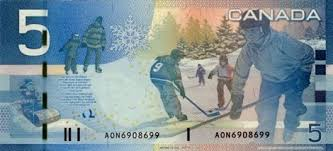
\includegraphics[width=0.50\textwidth]{canada5dollarbill.jpeg}
\end{center}

I understand that this 2004 poll is not a random sample.  However, these 
results suggest that hockey in Canada is a much larger part of the culture 
than any particular sport is in the USA (a non random online poll for the 
greatest Americans of all time at Ranker lists its first sports figure 
at 43, see:  
\url{https://www.ranker.com/list/greatest-americans-ever/jacariah}).  

It may be the case that the weighting methods that I propose might not hold 
up in the hockey example.  It is hard to know for sure since historical 
polling data for the popularity of sports in countries other than the US is 
hard to find.  It may very well be the case that hockey has five times the 
fan interest in Canada than it has in Russia.  Surveys indicate that 
football is the preferred sport in Russia 
(\url{http://russia.com/activity/football/}).  I agree that 
Sweden probably does not have twice the fan interest of Canada today, 
although hockey is very popular in Sweden 
(\url{https://en.wikipedia.org/wiki/Ice_hockey_in_Sweden}).  
The all-time rankings of hockey players are much more favorable to 
Canadians and they fall in alignment with the narrative presented, 
the origins of the sport (\url{https://en.wikipedia.org/wiki/Ice_hockey}), 
and nostalgia (see
\url{https://www.thescore.com/nhl/news/1361102}, 
\url{https://seatgeek.com/tba/sports/the-top-10-best-nhl-players-of-all-time/}, 
\url{https://www.thetoptens.com/hockey-players/}, 
and 
\url{https://www.nhl.com/fans/nhl-centennial/100-greatest-nhl-players}).


In any event, I do not think that the hockey analogy is an indictment 
of the weights that I employ as a sensitivity approach within the context of 
baseball.  Polling data on the changing popularity of baseball in the US is 
easy to obtain and goes back as far as 1937.  It is reasonable to suggest 
that this information can serve as a useful proxy in determining the MLB 
eligible population.  The weighting regime w3 is motivated from the following 
graph which is taken from Gallup polling data at 
\url{https://news.gallup.com/poll/4735/sports.aspx}

\begin{center}
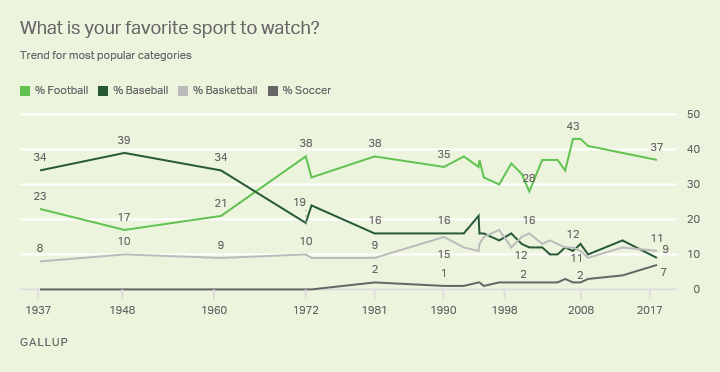
\includegraphics[width=0.75\textwidth]{Gallupfavoritesport.png}
\end{center}
%I can't say with certainty that this graphic captures the social fabric 
%component that baseball may have possessed in the earlier years of the 
%century.  However, 
This graphic is now added to the text.
%Intuitively, with no evidence -- 
%that baseball was played much more frequently, and was a much larger part of 
%the social fabric, in the earlier years of the century.  I've heard of kids 
%gathering at the sandlot to play pickup baseball games, but never football, 
%basketball, or hockey (in the US). 
The weighting regimes w1 and w2 are motivated from the Gallup article at 
\url{https://news.gallup.com/poll/6745/Baseball-Fan-Numbers-Steady-Decline-May-Pending.aspx?g_source=baseball%20interest&g_medium=search&g_campaign=tiles}
which notes that general interest in baseball has remained steady from 
1937 on.  This article is now added to the text.  This article and the above 
graphic suggests that it is a bit hyperbolic to state that baseball was 
played much more frequently, and was a much larger part of the social fabric, 
in the earlier years of the century.


I admit that the polling data only goes back to 1937, but I do not think that 
national interest in baseball was much different before 1937 than it was 
after.  For example as to why I think this, consider the 1927 Yankees which 
is one of the greatest baseball teams of all time, if not the greatest 
(\url{https://en.wikipedia.org/wiki/Murderers%27_Row}).  
However, the attendance 
figures for this great 1927 Yankees team were very modest in comparison to 
more modern Yankees seasons 
(\url{http://www.baseball-almanac.com/teams/yankatte.shtml})
even when taken relative to the population of New York City 
(\url{https://en.wikipedia.org/wiki/Demographic_history_of_New_York_City}).
Bleacher seat tickets at Yankee stadium cost anywhere from 50 to 75 cents  
in 1927 (\url{http://baseballguru.com/hfrommer/analysishfrommer80.html}) 
which is 7.10 to 10.65 in 2019 dollars. I do not think that cost is the 
explanation for modest attendance figures for the 1927 Yankees.  Also note 
that Yankees attendance is not limited by seating capacity 
(\url{http://www.baseball-almanac.com/stadium/yankee_stadium.shtml}).
Returning to hockey for a moment, in 1927 the Montreal Canadians had a much 
higher attendance than the Yankees relative to population 
(see \url{http://www.hockeydb.com/nhl-attendance/att_graph.php?tmi=6929} and 
\url{http://demographia.com/db-cancityhist.htm}).  The importance of hockey 
to Canadians is much greater than that of baseball to Americans. 


We are certainly taught that interest in baseball expanded in the roaring 
20s.  For example, see page 766 in the 8th grade history textbook 
\url{https://www.orange.k12.nj.us/cms/lib/NJ01000601/Centricity/Domain/434/United_States_History_Unit_8.pdf} 
used in Orange Public Schools in New Jersey.  
My freshman year history class taught the same thing, but I no longer 
have the textbook.
We do see an uptick in 
Yankees attendance starting in 1920 (this is the Babe Ruth season 
mentioned in the Introduction of the paper) which supports this narrative, 
but these figures are still modest in comparison to the attendance figures of 
more modern eras.  Additionally, there were no radio broadcasts of baseball 
games prior to 1920 
(\url{https://en.wikipedia.org/wiki/Major_League_Baseball_on_the_radio}).  
I do not think that interest in baseball could have been much larger before 
1920 considering that slugging Babe Ruth and the radio did not exist and 
attendance of baseball games was lower 
(\url{https://www.baseball-reference.com/leagues/MLB/misc.shtml}).  
Again, it is a bit hyperbolic to state that baseball was played much more 
frequently, and was a much larger part of the social fabric, 
in the earlier years of the century.

The anecdotal disappearance of sandlot baseball could partially be explained 
by the emergence of Little League baseball which started in 1939 and has 
greatly expanded ever since 
(\url{https://en.wikipedia.org/wiki/Little_League_Baseball}).

I think that the empirical evidence does support the use of the 
weighting regimes in the paper, especially in the manner in which they are 
used, and the interest in baseball compared to other sports in earlier times 
is picked up by these metrics.  
We also can clearly see that the weighting regimes were designed to address, 
and in fact, overcompensate for any potential shortcomings of no weighting.
%are chosen to be 
%antagonistic to the conclusions of the analysis with respect to the straight 
%population when reliable figures on baseball interest is missing.



%\bibliographystyle{plainnat}

%\bibliography{conjure}

\end{document}
